\section{The Weekplanner Application}\label{sec:TheWeekplannerApplication}

The following section describes the key elements of the Weekplanner application in an attempt to make the rest of the report clearer, as this report mainly consists of tasks completed on the Weekplanner application.

\subsection{Purpose}

Many people with an \gls{asd} need structure to function. Some \glspl{citizen} might need visual presentation\cite{VisualSupport} of their plans due to limited verbal communication skills. Fortunately for these people, there exist is a wide range of visual support tools for representing plans.

One of these support tools works with the help of pictures where each picture represents an activity in which the \glspl{citizen} should participate. Usually, the \glspl{guardian} organize the activities into days and the days into weeks, and as such, this tool is called the week-plan. We can see an example of such a week-plan in \autoref{fig:WeekPlan}.

\begin{figure}[H]
    \begin{center}
        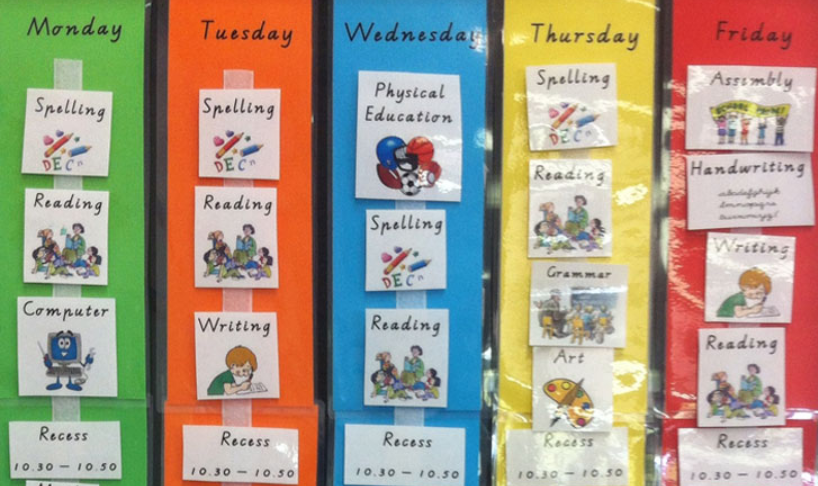
\includegraphics[width=0.95\textwidth]{figures/WeekPlanEks.png}
    \end{center}
    \caption{An example of a week-plan \cite{VisualSupport}.}
    \label{fig:WeekPlan}
\end{figure}

The \glspl{guardian} often use a board and tape the pictures onto it, which has some inherent problems. Firstly, moving the week-plan around and taking it along where ever the \gls{citizen} might go is immensely impractical. Secondly, the room on the board is limited, which means days can get full, which makes it difficult to add even more pictures to these days. Third, inserting pictures between others requires moving all pictures below the insertion point. Finally, with a limited number of pictures available, it is difficult to represent all the activities needed.

The \gls{giraf} customers requested an application with the same functionality as the original tool, but with more flexibility to use and edit, which is the goal of the Weekplanner application.

\subsection{Roles and Behaviors}

The week-plans has two types of users, \glspl{guardian} and \glspl{citizen}. Each week-plan is associated with a \gls{citizen}, but only \glspl{guardian}  modified it.

\subsubsection{Guardians}

\Glspl{guardian} are meant to control how the week-plans are laid out. \Glspl{guardian} can log into the system where they can get a list of \glspl{citizen} with whom they are working. When a \gls{guardian} chooses a \gls{citizen}, all of that \gls{citizen}'s week-plans are listed. The \gls{guardian} can then choose a specific week-plan which navigates to the chosen week-plan. The \gls{guardian} can then make changes to the week-plan or hand the week-plan over to the \gls{citizen} by switching to a more restrictive mode called \gls{citizen} mode.

\subsubsection{Citizens}

The \glspl{citizen} cannot log into the system. Instead, the \glspl{guardian} hand them the device after citizen mode is activated.

In citizen mode, \glspl{citizen} can mark the different activities as completed, but a citizen cannot change the week-plan or navigate the application. From citizen mode, a \gls{guardian} can switch the system back to guardian mode by providing a password.

\subsection{Application Screens}

The following section provides an overview of the different screens in the Weekplanner application as it were at the start of the semester. These screens are:

\begin{itemize}
    \item The \textit{Login screen},
    \item the \textit{Select Citizen screen},
    \item the \textit{Select Weekplan screen},
    \item the \textit{Weekplan screen},
    \item and the \textit{Find Pictogram screen}
\end{itemize}

\subsubsection{The Login Screen}

The \textit{Login screen} offers the ability to type in a username and a password, which can authenticate the user and then navigate to the \textit{Select Citizen screen}. We can see the layout in \autoref{fig:LoginProt}.

\begin{figure}[H]
    \begin{center}
        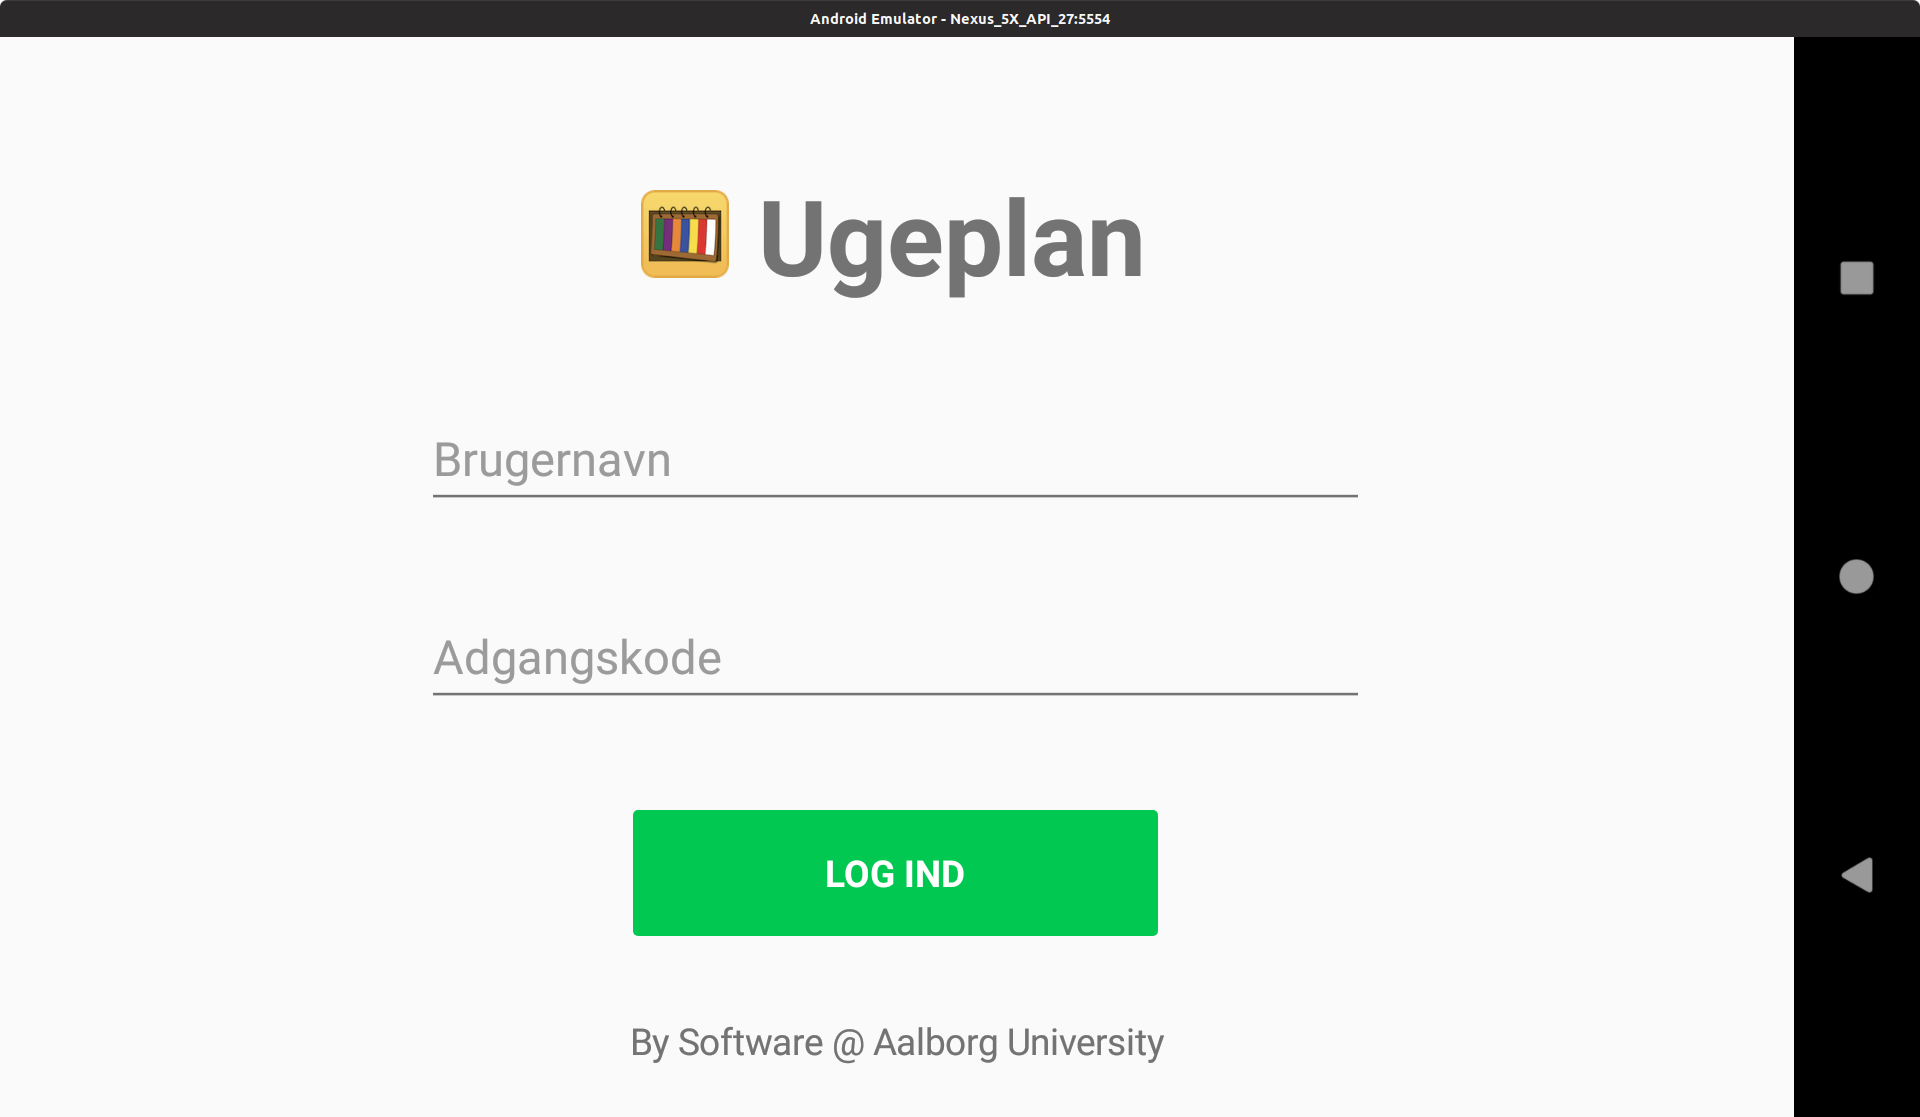
\includegraphics[width=0.7\textwidth]{figures/Prototypes/LoginScreenPrototype.png}
    \end{center}
    \caption{The \textit{Login screen}}
    \label{fig:LoginProt}
\end{figure}

\subsubsection{The Select Citizen Screen}

On this screen, the \gls{guardian} sees a list of the citizens under their care. When a \gls{guardian} wants to view a specific \gls{citizen}'s week-plan, they must first choose that \gls{citizen} from the list, which will bring up the available week-plans for that \gls{citizen} in the \textit{Select Week-plan screen}. We can see the layout in \autoref{fig:ChooseCitProt}.

\begin{figure}[H]
    \begin{center}
        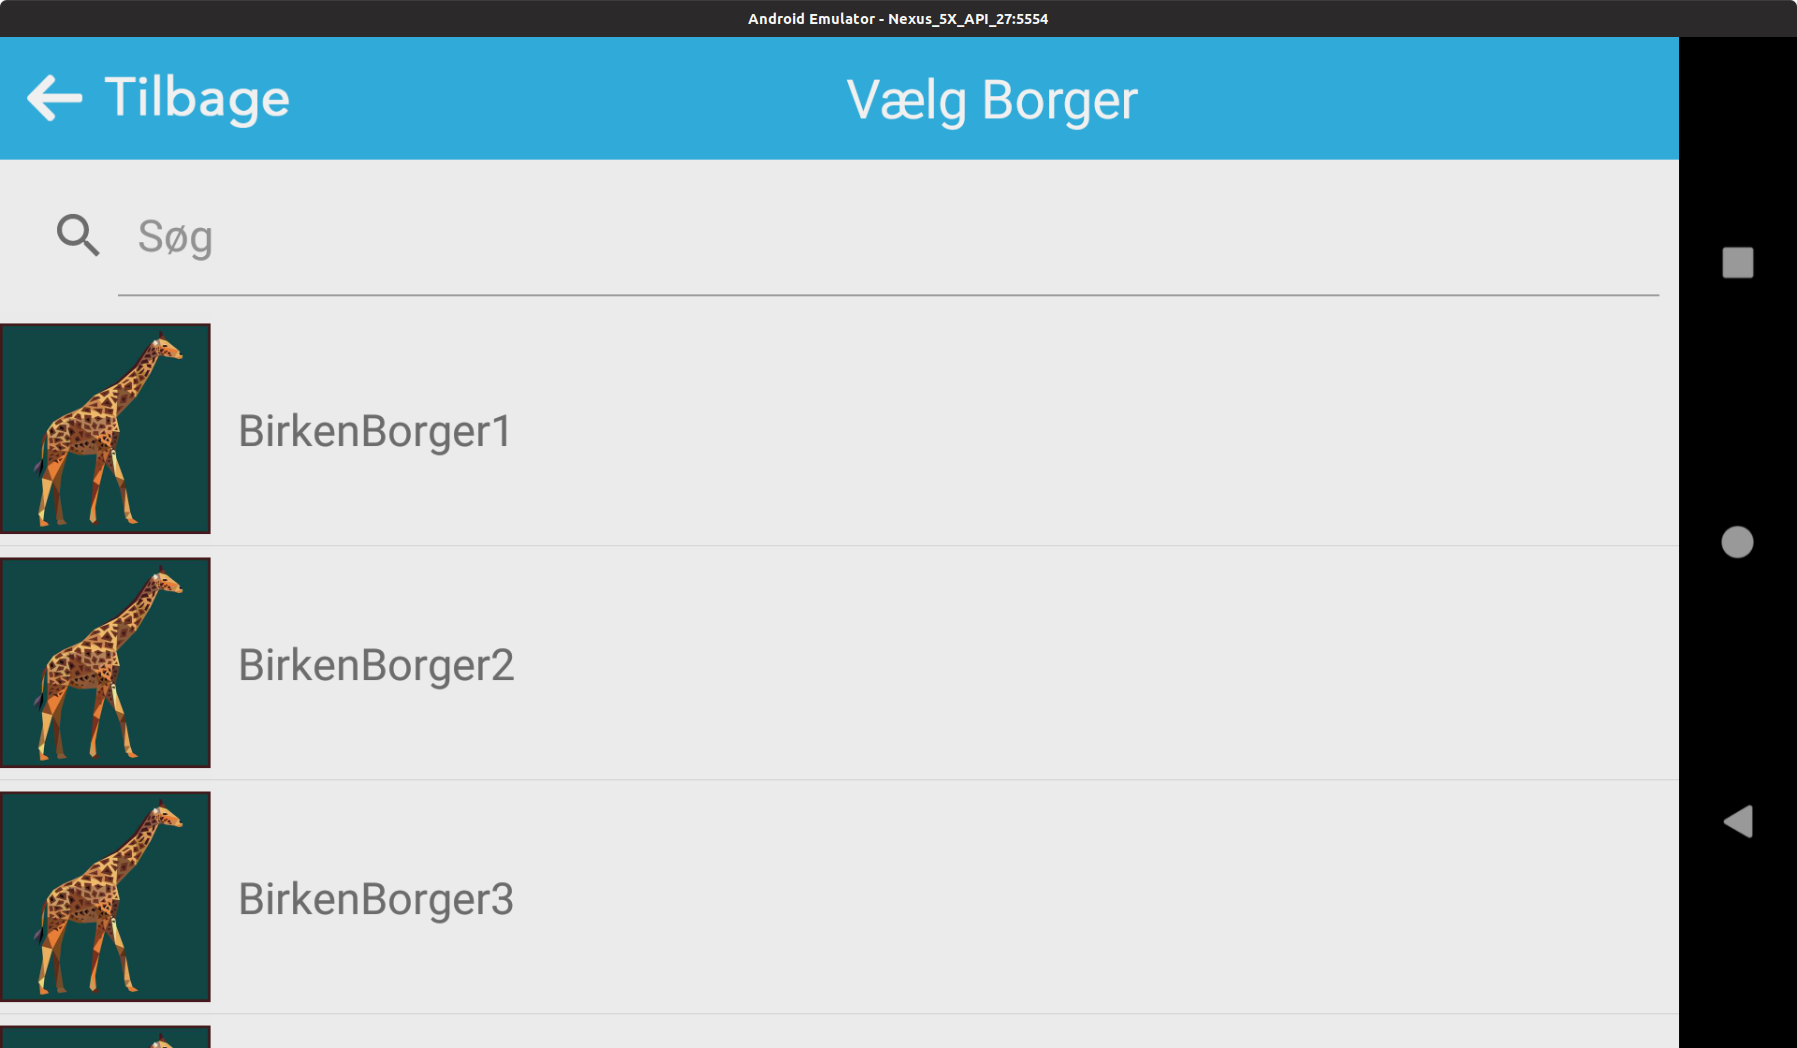
\includegraphics[width=0.7\textwidth]{figures/Prototypes/ChooseCitizenPrototype.png}
    \end{center}
    \caption{The \textit{Select Citizen screen}}
    \label{fig:ChooseCitProt}
\end{figure}

\subsubsection{The Select Week-plan Screen}

The \gls{guardian} can see a list of all week-plans belonging to the chosen \gls{citizen}. From here, the \gls{guardian} can select the desired week-plan. On the screen, there also is the ability to create a new week-plan for the citizen. We can see the layout in \autoref{fig:ChooseWeekProt}.

\begin{figure}[H]
    \begin{center}
        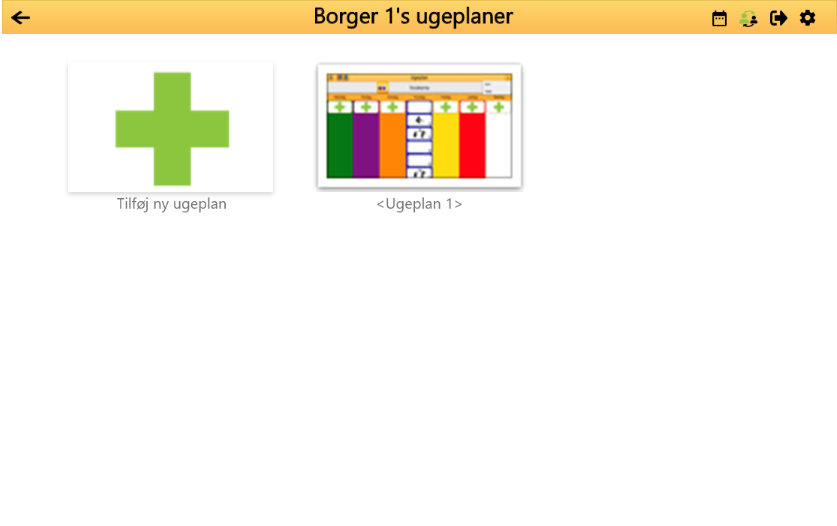
\includegraphics[width=0.7\textwidth]{figures/Prototypes/SelectWeekplanPrototype.png}
    \end{center}
    \caption{The \textit{Select Week-plan screen}}
    \label{fig:ChooseWeekProt}
\end{figure}

\subsubsection{The Weekplan Screen}

We can see the layout for the screen in both \gls{guardian} mode and \gls{citizen} mode in \autoref{fig:WeekplanProt}. In both modes, we can see the activities planned for the day. The difference between the two modes lies in the behavior exhibited by selecting an activity and in the ability to add additional activities to the screen. In \gls{guardian} mode selecting an activity navigates the the \textit{Edit Activity screen}, whilst in \gls{citizen} mode, the activity is marked as completed.

\begin{figure}%
    \centering
    \subfloat[Guardian]{{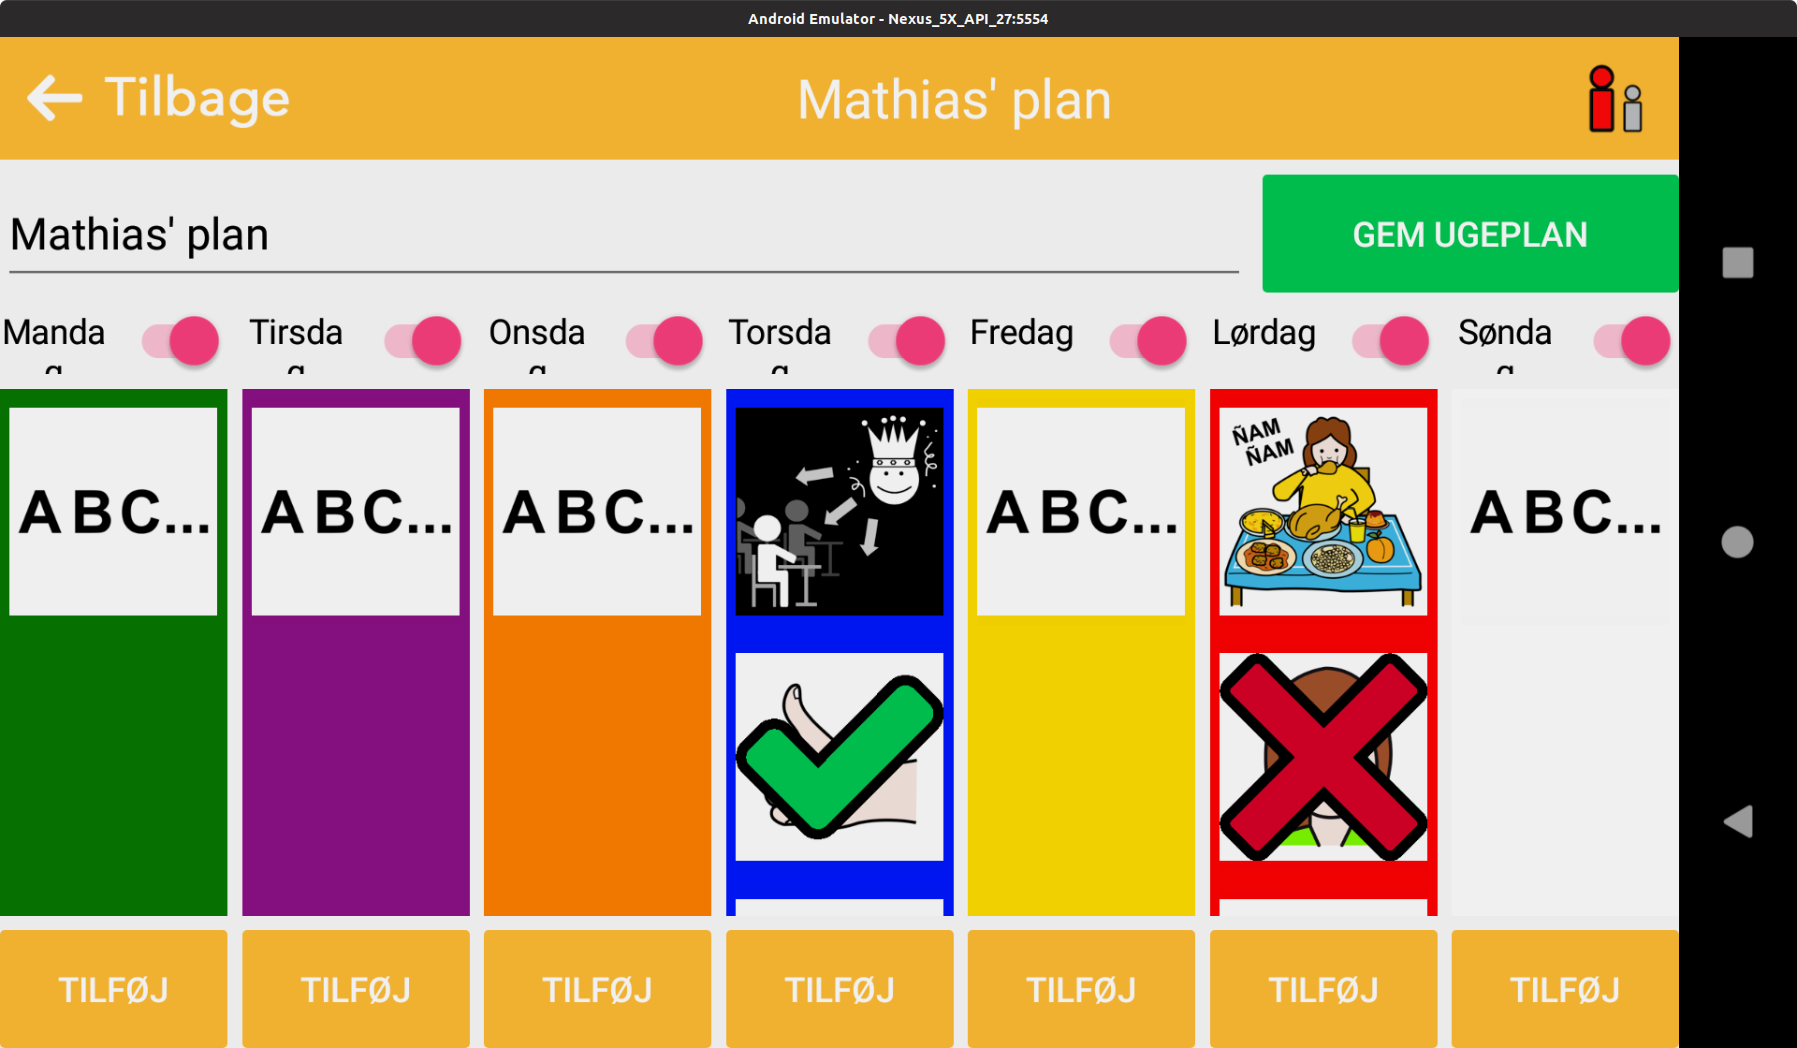
\includegraphics[width=0.65\textwidth]{figures/Prototypes/WeekPlannerGuardianPrototype.png} }}%
    \quad
    \subfloat[Citizen]{{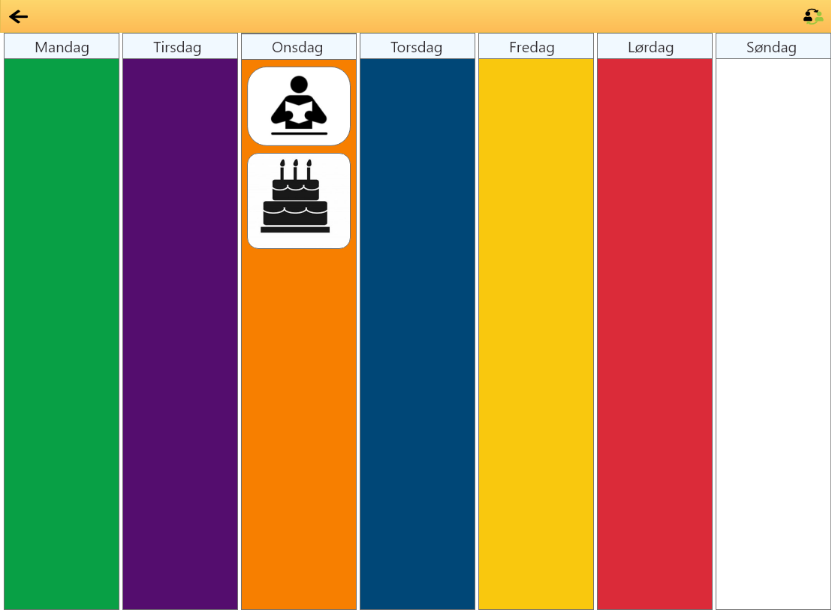
\includegraphics[width=0.25\textwidth]{figures/Prototypes/WeekPlannerCitizenPrototype.png} }}%
    \caption{The \textit{Week-plan screen} in the two different modes}%
    \label{fig:WeekplanProt}%
\end{figure}

% the old screens were:
% Activity Page
% Choice Board Page
% Choose Citizen Page
% Choose Template Page
% Citizen Schedules Page
% Login Page
% New Schedule Page
% Pictogram Search Page
% Settings Page
% Week-planner Page
% Week-planner Template Page

